 % -*- root: ../thesis.tex -*-
\chapter{Tensors}
\label{chap:tensors}

The theoretical and numerical study of many-body quantum systems is severely hindered by the \emph{curse of dimensionality}, which in this context refers to the exponential growth of the Hilbert space of quantum states w.r.t.\ the number of constituents.
However, many realistic systems do not exhibit this pathological complexity and can be described efficiently in terms of \emph{tensor networks}~\cite{}.
An especially simple but important special case of tensor networks is known under names such as \emph{finitely correlated states}~\cite{Fannes_1992_Finitely} or \emph{matrix-product states} (MPS)~\cite{Garcia_2006_Matrix,Verstraete_2008_Matrix,Orus_2014_Practical}.
\todo{Check this!}
Examples for quantum states that can be efficiently described as MPS include W-, GHZ-, and cluster states.
More generally, low energy states of one-dimensional gapped Hamiltonians with local interactions have an efficient MPS description and vice versa~\cite{}.
Here, \quotes{efficient description} refers to the fact that the number of parameters required to describe such a state scales polynomially in the number of subsystem.

The question we are attempting to answer in this chapter is whether such MPS can be efficiently reconstructed from few linear measurements\footnote{%
  Note that since we assume a linear measurement model, the results of this section do not apply to the problem of estimating pure quantum states.
  We use the term \quotes{matrix product state} to not only refer to quantum states, but to general tensors in the MPS format.
}.
More precisely, we provide evidence that the number of measurements required to recover a MPS is related to its intrinsic complexity -- and hence, scales polynomially in the number of constituents -- although its Hilbert space is exponentially large.
This work is a natural extension of \emph{low-rank matrix recovery}, which formed the foundation of the results in \cref{chap:phaselift}, to higher-order tensors.\\
\todo{tensors -> higher order, rank}

This chapter is structured as follows:
In \cref{sec:tensors.mps}, we introduce the MPS tensor format.
\Cref{sec:tensors.als} reports on work in progress, which is concerned with recovering MPS from few linear measurements using an \emph{Alternating Least Squares} (ALS) algorithm.
Finally, in \cref{sec:tensors.mpnum} we present the software library \mpnum dealing with tensors in MPS representation.
\mpnum was developed as part of this work to facilitate numerical computations in a user friendly and reusable manner.


\subsection*{Relevant publications}
\begin{itemize}
  \item Ž.\ Stojanac, D.\ Suess, M.\ Kliesch: \textit{On the distribution of a product of N Gaussian random variables}, Proceedings Volume 10394, Wavelets and Sparsity XVII; 1039419 (2017)
  \item Ž.\ Stojanac, D.\ Suess, M.\ Kliesch, \textit{On products of Gaussian random variables}, arXiv:1711.10516
  \item D.\ Suess, M.\ Holzaepfel, \textit{mpnum: A matrix product representation library for Python}, Journal of Open Source Software, 2(20), 465 (2017)
\end{itemize}
%%%%%%%%%%%%%%%%%%%%%%%%%%%%%%%%%%%%%%%%%%%%%%%%%%%%%%%%%%%%%%%%%%%%%%%%%%%%%%%%
\section{Matrix Product States}%
\label{sec:tensors.mps}

Tensors are a generalization of vectors and matrices.
Although there is a coordinate-free definition for tensors in terms of multi-linear forms~\cite{BROUWER?}, we are going to identify a tensor with it's coordinate representation here.
\todo{Also no distinguishing co/contravariant indices -> euclidean}
A complex tensor of order $N$ is an element $X \in \Complex^{d_1 \times \cdots \times d_N}$ and the $d_i$ are called \emph{local dimensions}.
Hence, a vector is a tensor of order 1 and a matrix is a tensor of order 2.
For the sake of simplicity, we assume that $d_1 = \cdots = d_N$ throughout this chapter.



\subsection{Graphical Notation}
\label{sub:mps.graphical_notation}

Since formulas with higher-order tensors may become incomprehensible due to the large amount of indices necessary, we introduce a common graphical notation~\cite{Dance,???}.
A tensor $X \in \Complex^{d^N}$ is represented by a geometric shape with legs attached, one for each index.
For example, consider the case $N = 3$, then
\[
  X_{i,j,k}
  =
  \begin{tikzpicture}[baseline=-.5ex]
    \tensor{{S=3, tensor_width=2, len_vertical_legs=0.5}}
    \node at (X) {$X$};
    \node [anchor=north] at (X_S1e) {\small $i$};
    \node [anchor=north] at (X_S2e) {\small $j$};
    \node [anchor=north] at (X_S3e) {\small $k$};
  \end{tikzpicture}
  .
\]
A variable written next to a leg fixes the corresponding index to the given value, while an anonymous tensor leg represents an unmatched index.
In the following, we will make use of the following notation for an unmatched index inspired by Python's and Matlab's syntax:
Given above $X \in \Complex^{d^3}$, we define the slice $X_{:,j,:} \in \Complex^{d^2}$ by
\[
  \label{eq:mps.slicing}
  X_{:,j,:}
  =
  \begin{tikzpicture}[baseline=-.5ex]
    \tensor{{S=3, tensor_width=2, len_vertical_legs=0.5}}
    \node at (X) {$X$};
    \node [anchor=north] at (X_S2e) {\small $j$};
  \end{tikzpicture}
  .
\]
For the components, we have the slightly cumbersome equality $\left(X_{:,j,:}\right)_{i,k} = X_{i,j,k}$.
The advantage of this graphical notation becomes clear once we express tensors composed of other tensors by operations such as index contraction or tensor products:
\begin{description}[font=$\bullet$\ \scshape\bfseries]
  \item[Contractions] are indicated by joining two legs, e.g.\ for matrices $A, B \in \Complex^{d \times d}$ their product $AB$ is written as
    \[
      \begin{tikzpicture}[baseline=-.5ex]
        \tensor{{W=1, E=1, tensor_name='AB'}}
        \node at (AB) {$AB$};
      \end{tikzpicture}
      =
      \begin{tikzpicture}[baseline=-.5ex]
        \tensor{{W=1, E=1, tensor_name='A'}}
        \node at (A) {$A$};
        \tensor{{W=1, E=1, tensor_name='B', x=1.25}}
        \node at (B) {$B$};
      \end{tikzpicture}
      :=
      \sum_k
      \left(
      \begin{tikzpicture}[baseline=-.5ex]
        \tensor{{W=1, E=1, tensor_name='A'}}
        \node at (A) {$A$};
        \node[anchor=west] at (A_E1e) {\small $k$};
        \tensor{{W=1, E=1, tensor_name='B', x=2.5}}
        \node at (B) {$B$};
        \node[anchor=east] at (B_W1e) {\small $k$};
      \end{tikzpicture}
      \right)
    \]

  \item[Tensor products] correspond to drawing two tensors side by side, e.g.\ for $x, y \in \Complex^d$ their tensor product $x \otimes y$ is written as
    \[
      \begin{tikzpicture}[baseline=-.5ex]
        \tensor{{S=2, tensor_width=1.5, tensor_name='xy'}}
        \node at (xy) {$x \otimes y$};
      \end{tikzpicture}
      =
      \begin{tikzpicture}[baseline=-.5ex]
        \tensor{{S=1, tensor_name='x'}}
        \node at (x) {$x$};
        \tensor{{S=1, tensor_name='y', x=1.25}}
        \node at (y) {$y$};
      \end{tikzpicture}
    \]

  \item[Grouping] indices -- that is the canonical identification $\Complex^{d_1} \otimes \Complex^{d_2} \cong \Complex^{d_1 d_2}$ -- is indicated by merging two or more legs together.
    \[
      \tikz[baseline=-.5ex]{\mpa{2}{{W=3, virtual=2, E=1}}}
      \cong
      \begin{tikzpicture}[baseline=-.5ex]
        \tensor{{W=1, E=1, len_horizontal_legs=0, tensor_name='A'}}
        \tensor{{W=1, E=1, len_horizontal_legs=0, tensor_name='B', x=1.25}}
        \draw[line width=2pt] (A_W1) -- +(-0.25,0);
        \draw[line width=1.5pt] (A_E1) -- (B_W1);
        \draw (B_E1) -- +(0.25,0);
      \end{tikzpicture}
      \label{eq:tensors.intro.grouping}
    \]
    This operation is often used in numerical implementations of tensor network algorithms as it reduces most tensor operations to standard matrix  operations.
    For example, the twofold contraction on the left hand side of \cref{eq:tensors.intro.grouping} is converted to a matrix multiplication on the right hand side.
    In the following, we often implicitly perform grouping on neighbouring tensor legs.
\end{description}



\subsection{MPS tensor representation}
\label{sub:mps.tensor_representation}

The tensor representation we are interested in has been established in quantum physics independently under the names \emph{finitely correlated states}~\cite{Werner} and \emph{matrix-product states}~\cite{Klumper}.
Subsequently, it has been rediscovered in other contexts:
It is known under the guise of the \emph{density matrix renormalization group}~\cite{White,Schollwoeck} in condensed matter physics.
Furthermore, the MPS representation is also known as a special case of the \emph{Hierarchical Tucker} tensor format~\cite{Hackbusch,Grasedyck} and under name \emph{tensor-train}~\cite{Oseledets_2011_TensorTrain} in the applied math community.
However, similar structures have been known for much longer in the form of \emph{deterministic finite automata}~\cite{Hopcroft} and \emph{hidden Markov models}~\cite{Baum}.

\todo{More motivation?}

To introduce the MPS representation, consider a tensor $X \in \Complex^{d^N}$.
By splitting off the first index, grouping the remaining $N-1$ indices, and performing a SVD on the resulting matrix, we can factor $X$ into three parts
\[
  \begin{tikzpicture}[baseline=-.5ex]
    \tensor{{S=4, tensor_width=3}}
    \node (X) {$X$};
    \draw[dashed] (-.6,-.8) -- (-.6, .8);
  \end{tikzpicture}
  =
  \begin{tikzpicture}[baseline=-.5ex]
    \tensor{{S=1, E=1, x=-3.3, tensor_name='L'}}
    \node at (L) {$M\ind{1}$};
    \tensor{{W=1, E=1, x=-2.1, tensor_name='lambda', tensor_style='tensornode, rounded corners=0.375cm, fill=red!30'}}
    \node at (lambda) {$\Lambda\ind{1}$};
    \tensor{{W=1, S=3, tensor_width=2.5, tensor_name='R'}}
    \node (R) {$\tilde R_{N-1}$};
  \end{tikzpicture}
\]
where $M\ind{1}$ denotes the left-singular vectors, $\Lambda\ind{1}$ the diagonal matrix composed of the singular values $\lambda\ind{i}$, and $\tilde R_{N-1}$ the left-singular vectors after the index-grouping has been reversed.
For convenience, we contract the singular values with the remainder $\tilde R_{N-1}$ and obtain
\[
  \begin{tikzpicture}[baseline=-.5ex]
    \tensor{{S=4, tensor_width=3}}
    \node (X) {$X$};
  \end{tikzpicture}
  =
  \begin{tikzpicture}[baseline=-.5ex]
    \tensor{{S=1, E=1, x=-2.1, tensor_name='L'}}
    \node at (L) {$M\ind{1}$};
    \tensor{{W=1, S=3, tensor_width=2.5, tensor_name='R'}}
    \node (R) {$R_{N-1}$};
  \end{tikzpicture}
\]
This procedure can now be iterated by performing the same steps on $R_{N-1}$:
\begin{align}
  \begin{tikzpicture}[baseline=-.5ex]
    \tensor{{S=4, tensor_width=3}}
    \node (X) {$X$};
    \draw[dashed] (-.6,-.8) -- (-.6, .8);
  \end{tikzpicture}
  &=
  \begin{tikzpicture}[baseline=-.5ex]
    \tensor{{S=1, E=1, x=-2.1, tensor_name='L'}}
    \node at (L) {$M\ind{1}$};
    \tensor{{W=1, S=3, tensor_width=2.5, tensor_name='R'}}
    \node (R) {$R_{N-1}$};
    \draw[dashed] (-.3,-.8) -- (-.3, .8);
  \end{tikzpicture}\\
  &=
  \begin{tikzpicture}[baseline=-.5ex]
    \mpa{{1,2}}{{S=1, E=1, x=-3.1, tensor_name='L'}}
    \node at (L_1) {$M\ind{1}$};
    \node at (L_2) {$M\ind{2}$};
    \tensor{{W=1, S=2, tensor_width=2}}
    \node (R) {$R_{N-2}$};
    \draw[dashed] (0,-.8) -- (0, .8);
  \end{tikzpicture}\\
  &=
  \begin{tikzpicture}[baseline=-.5ex]
    \mpa{4}{{S=1, tensor_name='L'}}
    \node at (L_1) {$M\ind{1}$};
    \node at (L_2) {$M\ind{2}$};
    \node at (L_3) {$M\ind{3}$};
    \node at (L_4) {$M\ind{4}$};
  \end{tikzpicture}
  \label{eq:mps.matrix_product}
\end{align}
This yields a representation of $X$ in terms of the \emph{local tensors} $M\ind{l}$.
The above algorithm for computing the local tensors is referred to as TT-SVD in \cite{Oseledets_2011_TensorTrain}.
In the following, we identify the index order as follows:
\[
  M\ind{l}_{i,j,k} =
  \begin{tikzpicture}[baseline=-.5ex]
    \tensor{{W=1, S=1, E=1}}
    \node at (X) {$M\ind{l}$};
    \node [anchor=east] at (X_W1e) {\small $i$};
    \node [anchor=west] at (X_S1e) {\small $j$};
    \node [anchor=north] at (X_W1e) {\small $k$};
  \end{tikzpicture}
\]
The horizontal, contracted legs corresponding to the indices $i$ and $k$, are often referred to as \emph{bond} or \emph{virtual legs} and the vertical, unmatched ones corresponding to $j$ are referred to as \emph{physical} legs.
By fixing each physical leg to some value $k_l$ in \cref{eq:mps.matrix_product}, we see that each component of $X$ is given by product of $N$ matrices
\[
  \label{eq:mps.local_matrices}
  M\ind{l}_{k_l} := M\ind{l}_{:,k_l,:},
\]
hence the name \quotes{matrix-product representation}.

%%%%%%%%%%%%%%%%%%%%%%%%%%%%%%%%%%%%%%%%%%%%%%%%%%%%%%%%%%%%%%%%%%%%%%%%%%%%%%%%
\begin{figure*}
  \centering
  \begin{tikzpicture}
    \tensor{{S=4, tensor_name='psi', tensor_width=3, tensor_height=1,
             len_vertical_legs=.5, x=-2.5}}
    \node at (psi) {$X_{ijkl}$};

    \node at (0,0) {\Huge $=$};

    \begin{luacode*}
      local indices = {'i', 'j', 'k', 'l'}
      -- local bond_indices = {'a', 'b', 'c'}

      mptikz.draw_mpa(4, {S=1, tensor_name='A', tensor_width=1, tensor_height=1,
                          len_vertical_legs=.5, len_horizontal_legs=.5, x=1.5})

      for i = 1, 4 do
        t('\\node[anchor=west] at (psi_S%i) {$%s$};', i, indices[i])
        t('\\node[anchor=west] at (A_%i_S1) {$%s$};', i, indices[i])
          t('\\node at (A_%i) {$M\\ind{%i}$};', i, i)
      end

      -- for i =1, 3 do
      --  t('\\node[anchor=north] at (A_%i_E1e) {$%s$};', i, bond_indices[i])
      -- end
    \end{luacode*}

    \draw[pointerline] (psi) -- +(2,-1) node[pointernode] {global tensor};
    \draw[pointerline] (A_2) -- +(1,1) node[pointernode] {local tensor};
    \draw[pointerline] (A_3_E1e) -- +(0.5,1) node[pointernode] {virtual leg};
    \draw[pointerline] (A_3_S1) -- +(-0.5,-0.5) node[pointernode,anchor=east] {physical leg};
  \end{tikzpicture}
  \caption{%
    \label{fig:mps.mps}
    A 4th order tensor in MPS representation with open boundary condition as described in \cref{eq:mps.open_boundary}.
  }
\end{figure*}
%%%%%%%%%%%%%%%%%%%%%%%%%%%%%%%%%%%%%%%%%%%%%%%%%%%%%%%%%%%%%%%%%%%%%%%%%%%%%%%%

So far this construction is exact and completely general, i.e.\ every tensor can be represented in MPS form, but not efficient:
Generically, the SVD in the $i$-th step yields $r_i = \min{d^i, d^{N - i}}$ non-zero singular values $\lambda\ind{i}$, and therefore, the local tensors $M\ind{i}$ have shape $(d, r_{i-1}, r_i)$.
However, suppose that all but $r$ of the singular values in each cut vanish, then we can truncate the local tensor $M\ind{i}$ to shape $(d, r, r)$.
In this case, the number of parameters scales as $\mathcal{O}(r^2 N d)$ and $X$ can be represented efficiently by matrix products according to \cref{eq:mps.matrix_product}.
Although this assumption may seem overly strict on a first glance, many tensors in our applications of interest are well approximated by such an MPS with small $r$.
The following definition sums up this section so far.

\begin{definition}%
  \label{def:mps.mps}
  A \emph{matrix-product state representation} of a tensor $X \in \Complex^{d^N}$ is defined in terms of a tuple of local tensors $(M\ind{l})_{l \in [N]}$ with $M\ind{l} \in \Complex^{r_{l - 1} \times d \times r_l}$ where $r_0 = r_N$.
  Then, the components of $X$ are given by
  \[
    \label{eq:mps.periodic_boundary}
    X_{i_1,\ldots,i_N} = \tr \left( M\ind{1}_{:,i_1,:}\ \cdots\  M\ind{N}_{:,i_N,:} \right).
  \]
  We say that the MPS representation has \emph{open boundary conditions} if $r_0 = r_N = 1$, otherwise the representation has \emph{periodic boundary conditions}.
\end{definition}

For the sake of simplicity, we restrict our attention to the open boundary case in the following.
In this case, we have
\[
  \label{eq:mps.open_boundary}
  X_{i_1,\ldots,i_N} = M\ind{1}_{i_1}\ \cdots\  M\ind{N}_{i_N},
\]
where we used the shorthand notation from \cref{eq:mps.local_matrices}
As already noted above, the crucial parameter balancing the efficiency of the MPS representation on one hand and its expressive power on the other hand is the size of the virtual legs $r_l$.
This warrants the following definition.

\begin{definition}%
  \label{def:mps.rank}
  Let $(M\ind{l})_{l \in [N]}$ denote an MPS representation with $M\ind{l} \in \Complex^{r_{l - 1} \times d \times r_l}$.
  We call $\max_l r_l$ the \emph{rank} or \emph{bond dimension} of the MPS.
  Furthermore, for any tensor $X$, we define its \emph{MPS-rank} to be the smallest rank of any MPS representation of $X$.
\end{definition}

Note that by~\cite[Thm.\ 2.2]{Oseledets_2011_TensorTrain}, the definition of MPS-rank in \cref{def:mps.rank} agrees with the usual definition using matrications of $X$, and hence, is well defined.\\


With the factorization of the tensor $X$ in \cref{def:mps.mps}, we have introduced new virtual degrees of freedom such that the partial trace over them equals $X$.
Clearly, the following gauge transformation leaves \cref{eq:mps.open_boundary} invariant
\begin{align}
  \tilde M\ind{1}_i = M\ind{1}_i R\ind{1},
  \tilde M\ind{N}_i = R\ind{N - 1} M\ind{N}_i, \\
  \tilde M\ind{l}_i = L\ind{l - 1} M\ind{l}_i R\ind{l} \quad (1 < l < N)
\end{align}
provided the (generally non-square) matrices $L\ind{l}$ and $R\ind{l}$ satisfy $L\ind{l} R\ind{l} = \1$ since then
\begin{equation}
  \begin{tikzpicture}[baseline=-.5ex]
    \mpa{4}{{S=1, tensor_name='A', len_horizontal_legs=0.1}}
    \node at (A_1) {$M\ind{1}$};
    \node at (A_2) {$M\ind{2}$};
    \node at (A_3) {$M\ind{3}$};
    \node at (A_4) {$M\ind{4}$};
  \end{tikzpicture}
  =
  \begin{tikzpicture}[baseline=-.5ex]
    \mpa{{1,4,7,10}}{{S=1,tensor_name='B', len_horizontal_legs=0.1}}
    \node at (B_1) {$M\ind{1}$};
    \node at (B_4) {$M\ind{2}$};
    \node at (B_7) {$M\ind{3}$};
    \node at (B_10) {$M\ind{4}$};
    \mpa{{2,5,8}}{{tensor_name='R', E=1, len_horizontal_legs=0.1, tensor_style='tensornode, fill=red!30'}}
    \node at (R_2) {$R\ind{1}$};
    \node at (R_5) {$R\ind{2}$};
    \node at (R_8) {$R\ind{3}$};
    \mpa{{3,6,9}}{{tensor_name='L', len_horizontal_legs=0.1, tensor_style='tensornode, fill=red!30'}}
    \node at (L_3) {$L\ind{1}$};
    \node at (L_6) {$L\ind{2}$};
    \node at (L_9) {$L\ind{3}$};
  \end{tikzpicture}
\end{equation}
As shown in~\cite[Thm. 2]{Perez-Garcia}, these local transformations on the virtual degrees of freedom are the only possible gauge transformations of the MPS representation.
A number of canonical forms exist that partially fix the gauge~\cite{Perez,Schollwoeck,Chubb}.
The following definition summarizes the corresponding gauge conditions

\begin{definition}%
  \label{def:mps.canonical}
  We say that a local tensor $M\ind{l}$ is \emph{left-normalized} if it satisfies
  \[
    \sum_k \adj{M\ind{l}_k} M\ind{l}_k = \1 \quad\quad\quad\quad
    \begin{tikzpicture}[baseline=-.5ex]
      \tensor{{W=1,S=1,E=1,tensor_name='A',y=0.5}}
      \tensor{{W=1,N=1,E=1,tensor_name='B',y=-0.5}}
      \draw[tensorleg] (A_W1e) -- (B_W1e);
    \end{tikzpicture}
    =
    \begin{tikzpicture}[baseline=-.5ex]
      \coordinate (A) at (0,0.5);
      \coordinate (B) at (0,-0.5);
      \draw[tensorleg] (A) -- (B);
      \draw[tensorleg] (A) -- +(.5,0);
      \draw[tensorleg] (B) -- +(.5,0);
    \end{tikzpicture}
  \]
  A MPS with all but the rightmost local tensors in left-normalized form is called \emph{left-canonical}.
  Similarly, a \emph{right-normalized} local tensor fulfills
  \[
    \sum_k M\ind{l}_k \adj{M\ind{l}_k} = \1 \quad\quad\quad\quad
    \begin{tikzpicture}[baseline=-.5ex]
      \tensor{{W=1,S=1,E=1,tensor_name='A',y=0.5}}
      \tensor{{W=1,N=1,E=1,tensor_name='B',y=-0.5}}
      \draw[tensorleg] (A_E1e) -- (B_E1e);
    \end{tikzpicture}
    =
    \begin{tikzpicture}[baseline=-.5ex]
      \coordinate (A) at (0,0.5);
      \coordinate (B) at (0,-0.5);
      \draw[tensorleg] (A) -- (B);
      \draw[tensorleg] (A) -- +(-.5,0);
      \draw[tensorleg] (B) -- +(-.5,0);
    \end{tikzpicture}
  \]
  and a \emph{right-canonical} MPS has all local tensors in right-normalized form except for the first.
\end{definition}

The exceptions for the local tensors at the beginning and end of the chain are necessary to accommodate tensors with Frobenius norm different from one.
In practice, we often deal with a mixed left-right-canonical form, e.g.\ in variational algorithms updating one local tensor at a time such as DMRG or the alternating least squares algorithm presented in \cref{sec:tensors.als}.
For these purposes, efficient algorithms exist that transform an MPS to a canonical form~\cite{schollwoeck,orus}.
If we neglect transformations that change the bond dimensions, the remaining gauge group is unitary, and hence, computations on canonical MPS are far more stable numerically.\\


We have already emphasized the ability of the MPS representation to represent certain tensors efficiently, i.e.\ with a number of parameters scaling polynomially in the order of the tensor.
One crucial advantage of this tensor format is that it also facilitates efficient arithmetical operations for tensors~\cite{Schollwoeck}.
In other words, operations such as sums and contractions of MPS are also MPS and the corresponding local tensors can be computed efficiently from the local tensors of the inputs.
For example, consider the scalar product of two tensors $A, B \in \Complex^{d^N}$:
\[
  \braket{A, B} =
  \begin{tikzpicture}[baseline=-.5ex]
    \mpa{3}{{S=1, y=.5, tensor_name='B'}}
    \mpa{3}{{N=1, y=-.5, tensor_name='A'}}
    \begin{luacode*}
      for i = 1,3 do
        t('\\node at (A_%i) {$A\\ind{%i}$};', i, i)
        t('\\node at (B_%i) {$B\\ind{%i}$};', i, i)
      end
    \end{luacode*}
  \begin{scope}[on background layer]
    \fill[tensornode,fill=black, opacity=0.1] ($ (A_1) - (0.5,0.5) $) rectangle ($ (B_1) + (0.5,0.5) $);
    \fill[tensornode,fill=black, opacity=0.1] ($ (A_2) - (0.5,0.5) $) rectangle ($ (B_2) + (0.5,0.5) $);
    \fill[tensornode,fill=black, opacity=0.1] ($ (A_3) - (0.5,0.5) $) rectangle ($ (B_3) + (0.5,0.5) $);
  \end{scope}
  \end{tikzpicture}
\]
By contracting the physical legs of the local tensors first as indicated by the gray boxes\footnote{%
  Note that this strategy is not optimal in many cases~\cite{schollwoecc} but suffices as an example here.
},
we obtain an MPS representation of a tensor of 0th order, i.e.\ a scalar, which can be contracted afterwards to compute its value.

As most arithmetic operations increase the virtual dimension substantially, we need methods to approximate the result by another MPS with lower virtual dimension while keeping the approximation error small.
Although computing the \emph{best} rank $r$ approximation of an MPS is computationally infeasible in general~\cite{Hillar_2013_Most}, there are efficient algorithms that produce good results in practice:
One of them is \emph{SVD compression}, which successively performs an SVD followed by a truncation of negligible singular values on the local tensors similar to the higher-order SVD introduced in \cref{eq:mps.matrix_product}~\cite{schollwoeck}.
If we truncate all but the $r$ largest singular values in each step, we obtain a quasi-optimal rank $r$ approximation of $X \in \Complex^{d^N}$, i.e.\
\[
  \norm{X - X_\mathrm{SVD}} \le \sqrt{N - 1} \norm{X - X_\mathrm{best}}.
  \label{eq:mps.quasi_optimal}
\]
Here, $\norm{\cdot}$ denotes the Frobenius norm of tensors, $X_\mathrm{SVD}$ the rank $r$ SVD compression, and $X_\mathrm{best}$ the best rank $r$ approximation of $X$.



\todo{Mention CANDECOMP/PARAFAC}
% \Cref{def:mps.rank} generalizes the notion of \quotes{matrix rank} to tensors of higher orders based on the MPS tensor format.
% Similar to the approach given in this section, the matrix rank can be defined in terms of a factorizing representation:
% The rank of a $d \times d$ matrix $X$ is the smallest integer $r$ such that $X$ can be written as a product of two $d \times r$ matrices $U$ and $V$:
% \[
%   A = U \adj{V}
%   \label{eq:mps.matrix_rank}
% \]
% Alternatively, the matrix rank can be defined in terms of sums of rank-1 matrices, i.e.\ as the smallest number of summands $r$ such that $X$ can be written as
% \[
%   A = \sum_{l=1}^r \ket{u\ind{l}} \bra{v\ind{l}}
%   \label{eq:mps.matrix_cannon_rank}
% \]
% with $u\ind{l}, v\ind{l} \in \Complex^d$.
% Of course, Eqs.~\eqref{eq:mps.matrix_rank} and \eqref{eq:mps.matrix_cannon_rank} are equivalent by the simple identification $u\ind{l} = U_{:,l}$ and $v\ind{l} = V_{:,l}$.

% The natural generalization of the matrix rank induced by \eqref{eq:mps.matrix_cannon_rank} to tensors of higher order is known as the \emph{canonical tensor rank}~\cite{Kolda_2009_Tensor}.
% For $X \in \Complex^{d^N}$, it defined as the smallest number of rank-1 tensors that add up to $X$:
% \[
%   X = \sum_{l=1}^r a\ind{l}_1 \otimes \cdots a\ind{l}_N, \quad a\ind{l}_i \in \Complex^d.
%   \label{eq:mps.canonical_decomposition}
% \]
% In other words, the canonical tensor rank is induced by the tensor decomposition~\eqref{eq:mps.canonical_decomposition}, which is known as \emph{CANDECOMP/PARAFAC}~\cite{Kolda_2009_Tensor}.
% In contrast to the matrix case, these two notions of tensor rank are not equivalent~\cite{}.

% Although it captures the natural structure of many problems~\cite{} and only requires $\Order(r N d)$ parameters, it has shortcomings in practice:
% First and foremost, computing the canonical tensor rank is $\NP$-complete~\cite{Hastad_1990_Tensor}.
% Furthermore, the best rank-$r$ approximation of a given tensor may not exist and it is also hard to compute if it exists~\cite{Hastad_1990_Tensor,Hillar_2013_Most,Lim}.
% In general, the CANDECOMP/PARAFAC decomposition is hard to deal with computationally.
% This is the reason why the MPS tensor format is becoming more popular.


\subsection{Applications of the MPS format}
\label{sub:mps.applications}

%%%%%%%%%%%%%%%%%%%%%%%%%%%%%%%%%%%%%%%%%%%%%%%%%%%%%%%%%%%%%%%%%%%%%%%%%%%%%%%%
\begin{figure*}[t]
  \centering
  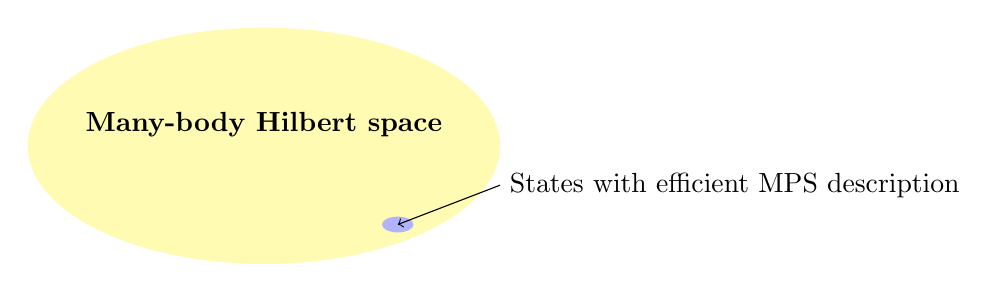
\begin{tikzpicture}
    \fill[fill=yellow!30,line width=0] (0,0) ellipse (3cm and 1.5cm) node[anchor=south] {\textbf{Many-body Hilbert space}};
    \coordinate (mpsstates) at (1.7, -1);
    \fill[fill=blue!30,line width=0] (mpsstates) ellipse (0.2cm and 0.1cm);
    \draw[<-] (mpsstates) -- (3,-0.5) node[anchor=west] {States with efficient MPS description};
  \end{tikzpicture}
  \caption{\label{tensors.mps_cartoon}%
    The manifold of quantum states with an efficient MPS description occupies only a tiny corner in the full Hilbert space.
  }
\end{figure*}
%%%%%%%%%%%%%%%%%%%%%%%%%%%%%%%%%%%%%%%%%%%%%%%%%%%%%%%%%%%%%%%%%%%%%%%%%%%%%%%%

% constitute variational classes of states that can efficiently parametrize interesting states such as...
%   -> linear local structure
%   - Link figure, area laws
%   - exponentially small corner, but very important, variational class of low-dimensiona
%   - time evolution stays there -> see Orus 3.4
%   - capture well physics
% on the other hand, also allow for an efficient implementation of crucial operations
% application in physics:
%   - fully described by order N tensor w.r.t. fixed PRODUCT basis <-> we'll identify the two
%   - captures entanglement structure of local interacctions
% case for states with strong area laws [citatoin], but generally every state with an area law can be approximated arbitatarly well with bond dimension scaling polynomially in N -> efficient description!


% generalizations:
%   - MPO -> 2 legs per site -> useful to describe multi-body mixed states -> positvity hard [Kliesch], but more expressive [Cuevas]
%   - PMPS -> local purification such that tracing out aux legs gives mixed states -> guaranteed to be positive
%   - in mpnum -> general data strucutre -> MPArray -> arbitatary legs per site




%%%%%%%%%%%%%%%%%%%%%%%%%%%%%%%%%%%%%%%%%%%%%%%%%%%%%%%%%%%%%%%%%%%%%%%%%%%%%%%%
\section{The Python Library mpnum}%
\label{sec:tensors.mpnum}


%%%%%%%%%%%%%%%%%%%%%%%%%%%%%%%%%%%%%%%%%%%%%%%%%%%%%%%%%%%%%%%%%%%%%%%%%%%%%%%%
\section{ALS for Tensors}%
\label{sec:tensors.als}

\subsection{Introduction}
\label{sub:tensors.als.introduction}

In the last chapter, we discussed a solution to the phase retrieval problem based on ideas from \emph{low-rank matrix recovery}.
The latter can be summarized as follows.
Consider a matrix\footnote{%
  Here, we choose $X$ to be real to simplify some notation -- an adaption of the statements made to the complex case is straight forward.
}
$X \in \Reals^{d \times d}$ of rank $r$, i.e.\ $X$ has only $r$ non-zero singular values.
The goal is to reconstruct $X$ from $m$ linear measurements of the form
\[
  y_l = {\braket{A\ind{l}, X}}, \quad l=1,\ldots,m
  \label{eq:tensors.lin_measurements}
\]
where $\braket{A, B} = \tr (\transpose{A} B)$ denotes the Frobenius inner product, $A\ind{l} \in \Reals^{d \times d}$ the \emph{measurement matrices}, and $y_l \in \Reals$ the corresponding measurement data.
In other words, we are looking for a solution $X$ of the linear problem defined by \cref{eq:tensors.lin_measurements}.
Note that \cref{eq:tensors.lin_measurements} describes the idealized measurements in the absence of noise.

In case the $A_i$ span $\Reals^{d \times d}$, this can be solved simply by computing the (pseudo-)inverse similar to \cref{sub:ortho.linear_inversion}.
However, in the underdetermined case $m < d^{2}$, this constitutes an ill-posed linear problem.
Nevertheless, we can still single out a unique solution in some cases by exploiting the additional structure, namely the low-rank assumption.
For example, in \cref{thm:FIXME} we show that $m = \Order(d)$ random measurements sampled from an appropriate distribution are sufficient to reconstruct any positive semidefinite, Hermitian $X \in \Complex^{d \times d}$ with unit rank.
More generally, we can recover any $X \in \Reals^{d \times d}$ with $\rank X = r$ from $m = \Order(d r)$ randomly chosen measurements~\cite{Candes_2011_Tight,Kueng_2014_Low}.
Intuitively, this sample complexity is asymptotically optimal since we need at least $2 d r$ real parameters to specify the left- and right-singular vectors of $X$, see~\cite{Eldar_2012_Uniqueness,Li_2017_Optimal} for rigorous lower bounds.

But \cref{thm:FIXME} not only guarantees identifiability of $X$, it also provides a semidefinite program to compute the reconstruction.
\todo{Why is this solution?}
The existence of such an efficient algorithm is crucial since the straight-forward reconstruction via rank minimization
\[
  \estim{X} = \argmin_{X'} \rank X' \quad\mathrm{s.t.}\ \braket{A\ind{i}, X'} = y_i (i = 1, \ldots, m)
\]
is $\NP$-hard~\cite{Mesbahi}.\\

A closely related problem is studied under the name of \emph{compressed sensing}:
The goal is to recover an $s$-sparse vector $X \in \Reals^d$ from linear measurements as in \cref{eq:tensors.lin_measurements} with $\braket{\cdot, \cdot}$ denoting the Euclidean scalar product on $\Reals^d$.
Here, a vector is $s$-sparse if it has $s$ non-vanishing components with respect to a certain basis.
Therefore, the property of having low-rank may be regarded as a non-commutative analogue of sparsity since a matrix has low-rank if and only if it is sparse in its eigenbasis.
\todo[noline]{Check log factors}
Similar to the matrix case, $X$ can be recovered from $m = \Order(s \log d)$ randomly chosen measurement vectors $A\ind{l} \in \Reals^d$ using a linear program~\cite{Foucart_2013_Mathematical}.
Hence, the number of measurements required scales with the \emph{intrinsic complexity} of the sparse signal vector:
If we encode each component of $X$ using $N$ bits, we can encode the full vector using
\[
  N \times s + s \log d = \Order(s \log d)
\]
bits.
The second summand on the left hand side is necessary to encode the positions of the non-zero components.

In conclusion, both compressed sensing and low-rank matrix recovery provide techniques to efficiently reconstruct a low-complexity, compressible signal embedded in a higher-dimensional space from linear measurements.
Here, \quotes{efficiently} refers to both, low computational as well as sample complexity -- that is the number of measurements required scales with the intrinsic complexity of the signal and not the dimension of the ambient space.\\



In this chapter, we consider a natural extension of the ideas introduced above to the problem of recovering low-rank tensors.
For this purpose, consider a tensor $X \in \Reals^{d_1 \times \cdots \times d_N}$.
If not stated otherwise, we assume $d_1 = \cdots = d_N = d$ throughout this chapter.
Contrary to the case of matrices, there are many inequivalent definitions of \quotes{rank} for tensors.
The most natural generalization of the matrix rank is given by the \emph{canonical tensor rank} of $X$, which is defined by the smallest number of rank-1 tensors that add up to $X$~\cite{Kolda_2009_Tensor}
In other words, the canonical tensor rank is the smallest number $r$ such that
\[
  X = \sum_{l=1}^r a\ind{l}_1 \otimes \cdots a\ind{l}_N
  \label{eq:tensors.canonical_decomposition}
\]
with $a\ind{l}_i \in \Reals^{d_i}$.
The decomposition~\eqref{eq:tensors.canoncial_decomposition} is known under many names such as \emph{CANDECOMP/PARAFAC}~\cite{Kolda_2009_Tensor}.
Although it captures the natural structure of many problems and only requires $\Order(r N d)$ parameters, it has shortcomings in practice:
First and foremost, computing the canonical tensor rank is $\NP$-complete~\cite{Hastad_1990_Tensor}.
Furthermore, the best rank-$r$ approximation of a given tensor may not exist~\cite{Kolda_2009_Tensor} and it is also hard to compute if it exists~\cite{Hillar_2013_Most}.
In general, the CANDECOMP/PARAFAC decomposition is hard to deal with computationally.
\todo{Some compressed sensing results for canonical low-rank tensors}

A different notion of tensor rank is induced by the tensor decomposition known under many different names such as \emph{matrix-product states} (MPS)~\cite{Garcia_2006_Matrix,Verstraete_2008_Matrix,Orus_2014_Practical} and \emph{finitely correlated states}~\cite{Fannes_1992_Finitely} in quantum physics or \emph{tensor train} (TT)~\cite{Oseledets_2011_TensorTrain} in the applied math community.
We introduce the exact definition in \cref{sec:tensors.mps}, but let use point out that a tensor $X \in \Reals^{d^{\otimes N}}$ with MPS-rank $r$ can be parametrized by $\Order{r^2 N d}$ real numbers.
This motivated the main question we are trying to answer in this chapter:
Can we efficiently reconstruct a tensor with low MPS-rank from few linear measurements?
In the ideal case, the number of measurements required for reconstructing a tensor with low MPS-rank would scale as $m = \Order{r^2 N d}$, which is an exponential improvement over the naïve linear inversion requiring $m = d^N$.
In contrast, compressed sensing or low-rank matrix recovery techniques can only yield polynomial improvement in the sample complexity.


%
% big problem: standard model (fully Gaussian measurements) also not efficient; partially solved in Zeljka

\subsection{Theory}%
\subsection{Numerics}%
% Implementation details; how to speed up initialization, why suitable for GPU%

